\chapter{Minority games}
\label{chapter:minority}

Minority games (MG) is a simple multi-agent based approach to simulating financial markets. 
It was first introduced by Challet and Zhang in \cite{challet1997emergence}, and has since evolved in it's many forms.
Although it has been mainly used to simulate financial markets, with certain modifications this model can be used to simulate any kind of system where agents act independently and in their best interest, while the resource for which they are competing is limited.
Humans and machine solve these kinds of problems everyday and some of the example are the choice of a road to take to evade traffic, or the routing a packet takes in the network to evade delays.

Main idea behind minority games is that each agent acts in his own best interest by following a certain set of strategies defined for each agent.
These strategies are deterministic, and each agent has a number of them.
It has been noted that the number of strategies per agent, as long as it is greater than one, has no effect on the qualitative properties of the model, so in most works it is enough to give two strategies per agent to test various hypothesis.

The agents use the history of the game to decide at each round which action to compute, $A$ or $B$, and the history itself is generated by the agents.
At each round a minority is calculated and is defined as a winning side, so if fewer agents have chosen $B$ as their action it becomes the winning side, and all the agents and strategies that have made that decision are awarded points.

Most of the economics models are deductive in nature and have proven difficult to analyse with conventional physicist models.
Since the agents in minority games are inductive, the model has proven popular among physicists to study and analyse financial markets by using some conventional physicists models \cite{yeung2009minority}.

Another major feature of the MG model are two distinctive phases which characterize the game.
In the two phases there are clearly different collective behaviours of the agents that can be explained by the quantity and cognitive abilities of the agents.

Further noted is the fact that with a simple model as this, and small modifications, various financial market characteristics are observable.
Macroscopic behaviour characteristic of financial markets, such as fat tail price return as volatility clustering, can be observed in MG models.
Aside from allowing a macroscopic analysis of the simulated financial markets, minority games offer an opportunity to study the microscopic properties, mainly how the decision-making process used by every agent. 
All of these aspects have made minority games popular among physicists interested in the study and analysis of financial markets, and have brought around a new field of research known as econophysics.

There are certain variations that have been proposed in literature to bring the model even closer to the financial markets.
One of the main versions of the game is Grand Canonical MG, that adds the possibility for agents to abstain from the market if they find the game unfavourable to them.
Due to the simple nature of the basic model there is great freedom in modifying the behaviour of the agents and thus the model, and many variations are available in the academic literature.

In this chapter we describe the basic model of the game \ref{minority:basicmodel}, give a more detailed definition in subsection \ref{minority:definition}. After that we explain the major features of the model in \ref{miinority:majorfeatures}, and conclude the chapter with two subsections that introduce the variations of the model used to simulate financial markets in \ref{minority:variations} and our own model that add the vicinity structure to the game in \ref{minority:vicinity}.

\section{The Basic Model}
\label{minority:basicmodel}

The basic model of the minority games are based on the El Farol Bar problem, defined by Brian Arthur in \cite{arthur1994inductive}.
In the El Farol community every Thursday there is a cultural event that people like to attend.
However if more that $60\%$ of the population goes to the Bar they will not have fun for it is overcrowded, and a better decision would be to have stayed home.
If less than $60\%$ of the population is present at the Bar than the will have good time, and staying at home is considered a less favourable decision.
Every person has to decide independently based only on their knowledge of past week.
This makes their behaviour inductive, as they can only remember a finite amount of weeks and the attendance at the bar.
The agents act in their own best interest and try to predict every week what the attendance will be at the bar, and then decide whether to attend or stay at home.
This model is also self contained as the new information, ie. the attendance at the bar in current week, is generated by the population.

This idea has been modified by Challet and Zhang into the first model of Minority Games.
Mainly the limit for deciding the winning side has been lowered to $50\%$, which makes the winning side the minority one, hence the name Minority Games.
The use of MGs as a model to simulate financial markets is justified by a simple consideration of the nature of economic system.
The basic assumption in the system is the supply and demand phenomenon.
This economic concept explain that when the supply is high, the price will be driven low so it is considered a good choice to buy.
Viceversa, if the demand is high it will drive the price high and a strategy to sell is considered good.
This simple mechanism, to buy or sell based on the fact whether other participants of the market are buying or selling is perfectly simulated by the minority rules.

\section{Definition of the Model}
\label{minority:definition}

The model is defined as a set of $N$ agents, where $N$ is an odd integer.
This constrain is used to be able to determine the minority side.
Population of agents is involved in a series of repeated games where at each round every agent has to make a choice between two actions.
These to actions can model various resources, as mentioned in \ref{1:competitive}, and in the case of computational representation we have chosen to use "0" and "1".
Note that in some literature the convention for simulating minority games is to use "-1" and "1" as the opposed actions possible, hence some definitions have to be change to reflect a different choice representation.
The action that the agent takes at step $t$ is also referenced as \textit{bid} in literature and is denoted by $a_i(t)$, corresponding to the bid of the agent $i$ at time $t$.

Each agent makes his decisions based on a set of strategies that are available. When the game starts agents draw a number of strategies, equal to $S$, from the set of available strategies.
A strategy is defined as a discrete function, $f:2^M\to\{0,1\}$, where $M$ is the \textit{memory} or the \textit{brain size} of each agent.
The memory represents how much past information can each agent store and use in order to predict future outcomes.
An example strategy of brain size $3$ can be seen in \ref{table:minorityStrategy}.
For a game with memory $M$ the total amount of possible signals is $2^M$, hence the total number of strategies in the strategy pool is $2^{2^M}$.

The history, denoted as $\mu(t)$, is a string of $M$ bits that records the winning actions of the past $M$ steps.
It is also called the \textit{information} as it can be of external or internal origin, or be a mix of the two.
So if an agent is using this strategy defined in \ref{table:minorityStrategy} to predict future outcome, and the \textit{information} is $'101'$, it will predict that the next correct action should be $1$.
Of course, to see whether this action is really the winning action we have to look at the decisions made by all the agents.

The sum of all the agent's decisions is called \textit{attendance}, denoted as $A(t)$ and defined as:
\begin{displaymath}
A(t)=\sum_{i=1}^N a_{i,s_i}^{\mu(t)}(t) = \sum_{i=1}^N a_i(t)
\end{displaymath}
Where $a_{i,s_i}^{\mu(t)}(t)$ is the decision made by agent $i$ at time $t$ using the best strategy $s_i(t)$ with the information $\mu(t)$.

To define how the best strategy is calculated between $S$ strategies of the agent, we first need to introduce the concept of \textit{cumulated payoff}, referred also as \textit{virtual score }of the strategy. 
The idea behind the virtual score is to follow the decision making of the strategy through time, whether it is used or not, and confront it to the winning choices.
If the strategy predict the winning side correctly, even if it is not used, it is rewarded a certain amount known as \textit{payoff} to it's virtual score, hence the name cumulated payoff.
Viceversa, when the strategy makes an erroneous prediction same amount is detracted from it's cumulated payoff.
This way agent can see which strategy would have brought him best win ratio over time, and chooses to use it in the next step. 
If more than one strategy has the maximum virtual score at time $t$, then one of the best strategies is chosen randomly.
The best strategy is defined as:
\begin{displaymath}
s_i(t) = \argmax_s U_{i,s}(t)
\end{displaymath}
Where $U_{i,s}(t)$ is the cumulated payoff of strategy $s$ of agent $i$.
This parameter starts from an arbitrary value, usually zero, and is defined as:
\begin{displaymath}
U_{i,s}(t+1) = U_{i,s}(t) -  \sign[( 2 a_{i,s}^{\mu(t)}(t+1) - 1 )(A(t) - \frac{N}{2}  )]
\end{displaymath}
Note that the convention we are using for representing actions is "0" and "1" so our attendance is always positive and has to be confronted with $\frac{N}{2}$.
Same goes for the agents action that should be brought to the "-1" and "1" representation to be able to calculate whether the agent made the winning decision.
If we were using the $(-1,1)$ convention we could calculate the cumulated payoff at time $t+1$ with
\begin{displaymath}
U_{i,s}(t+1) = U_{i,s}(t) -  \sign[a_{i,s}^{\mu(t)}(t+1) A(t) ]
\end{displaymath}

With the mechanism of choice between different strategies each agent becomes adaptive.
Of course there is a problem with randomly drawing strategies for it is possible for an agent to draw two very similar strategies and hence cannot use the information to it's fullest as his strategies act in similar fashion.

Being the total number of agents equal to an odd integer, a minority side can be calculated at each step.
As the number of winner is always smaller than the number of losers the minority game is a \textit{negative-sum-game}.
Since the two actions are symmetric it can be noted that the average of attendance over time is equal to $\frac{N}{2}$ (or $0$ when $(-1,1)$ convention is used).
It is therefore more interesting to study other moments of the model, mainly the fluctuation of attendance.
The variation of attendance is defined as
\begin{displaymath}
\sigma^2 = \langle A^2 \rangle - \langle A \rangle^2
\end{displaymath}
It is one of the main parameters when studying minority games, and has been proven that the variance of attendance in a model is not influenced by the source of information.
So whether an exogenous or an endogenous model is simulated the observed properties of the variance remain the same.

\section{Major features}
\label{miinority:majorfeatures}
Most important feature of the minority game model  is the characteristic two phases that occur described in \ref{subsec:phasetransition}, but first we describe the logical approach took to define the control parameters of this phenomenon.

\subsection{Standard deviation of attendance}
\label{subsec:stddev}

As the average of the attendance of a basic model tends to $\frac{N}{2}$ as noted in \ref{minority:definition} it is not very useful when studying the model.
There are two major aspect that can be studied in the model, $M$ and $N$ that respectively represent the memory of the agent and the total number of agents.
One can choose to study what happens when cognitive abilities of agents change, ie. the quantity of information that can be remembered and processed.
Let's assume that $N$ is fixed, and that we vary $M$ within certain interval.
One simple value that we can track is the standard deviation of attendance.
The graph of standard deviation against brain size is shown in figure \ref{fig:memory to stddev}.
The data have been generated using basic minority model, with $N=101$ and $M\in[2,12]$.
We have done in total 32 runs to be able to see the trend in the data.

\begin{figure}
\begin{center}
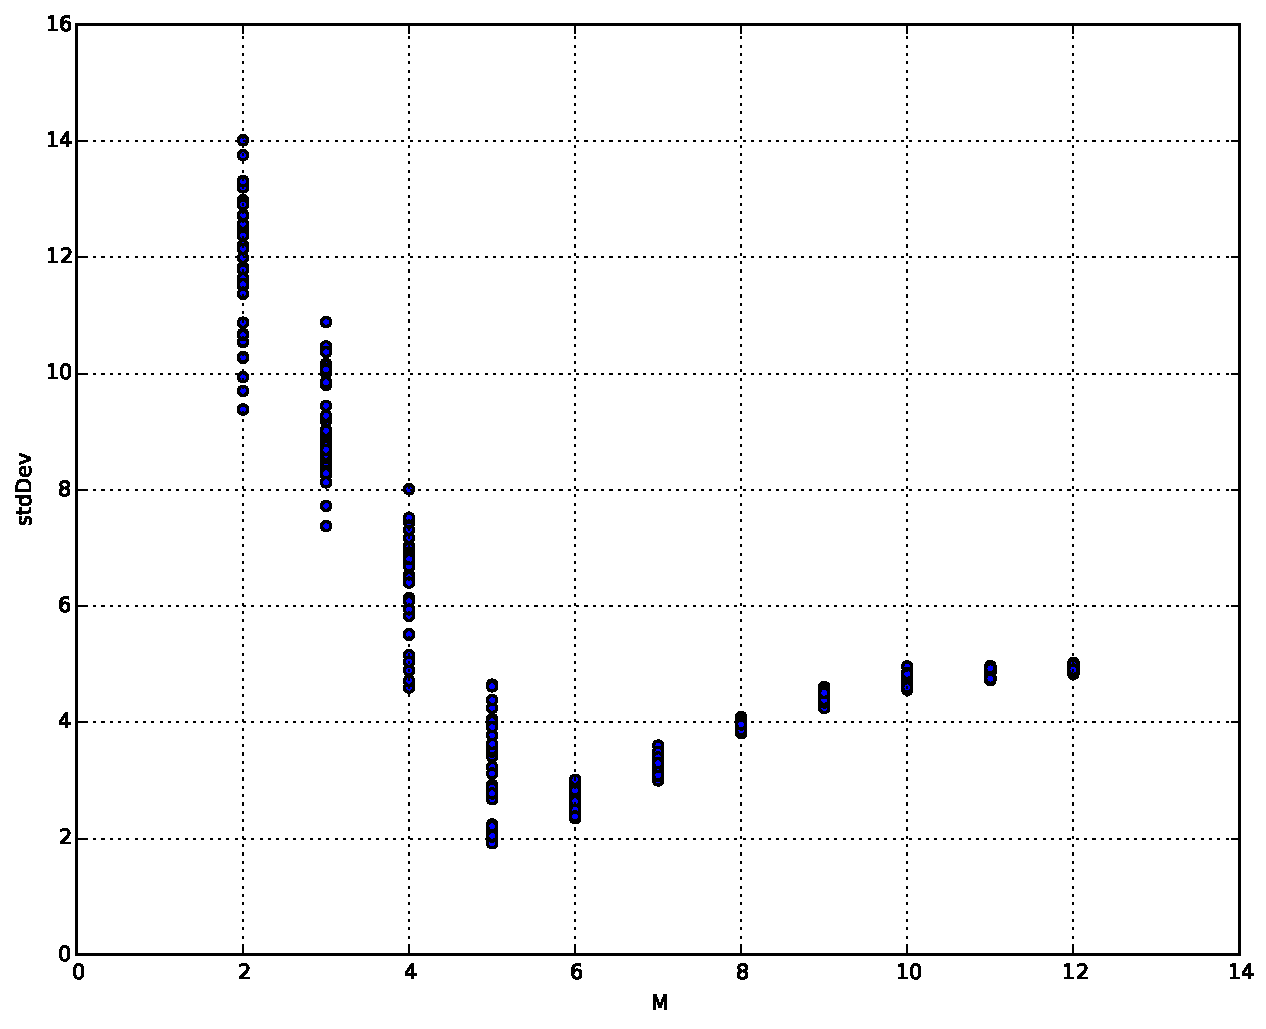
\includegraphics[scale=0.4]{images/minority/memory_to_stddev.pdf}
\caption{Plot of standard deviation of attendance for a model with 101 agents and 32 runs. In the axis memory (brain size) of agents}
\label{fig:memory to stddev}
\end{center}
\end{figure}

We can see that there is a minimum of the function somewhere between value $5$ and $6$ for memory.
Before this point standard deviation is definetly high with respect to the rest of the graph, and after the critical point it seems to converge to some value.

It is already evident that there is certain connection between the memory of agents and their ability to perform efficiently, intended as a efficient distribution of the resource they are competing for.
In this graph however $N$ is a fixed value, so let us see what happens when we start varying both parameters. 

\subsection{Phase Transition}
\label{subsec:phasetransition}

After further studies Savit, Manuca and Riolo \cite{savit1999adaptive} have noted that the macroscopic behaviour of the model does not depend independently on the single parameters $M$ and $N$, but rather on the rapport between the two.
They have discovered that a new control parameter $\alpha$ defined as $\alpha=\frac{2^M}{N}$ defines the volatility of the model.
Volatility is defined as a normalized variance:
\begin{displaymath}
\frac{\sigma^2}{N}
\end{displaymath}
The volatility depends only on the ratio between $2^M$ and $N$ and it is no influenced by the source of information, meaning that it maintains it's characteristic behaviour in endogenous and exogenous games.

In figure \ref{fig:normalized variance} volatility is plotted versus the control parameter $\alpha$.
The red line in the graph represents the volatility of a \textit{random-choice} model.
If we create a model where all the agents make random decision at every step the volatility that we obtain is:
\begin{displaymath}
\frac{\sigma^2}{N} = \frac{Np(1-p)}{N} = 0.5(1-0.5) = 0.25
\end{displaymath}
This is calculated assuming a binomial distribution of agent's actions with probability $p=0.5$.

\begin{figure}[h]
\begin{center}
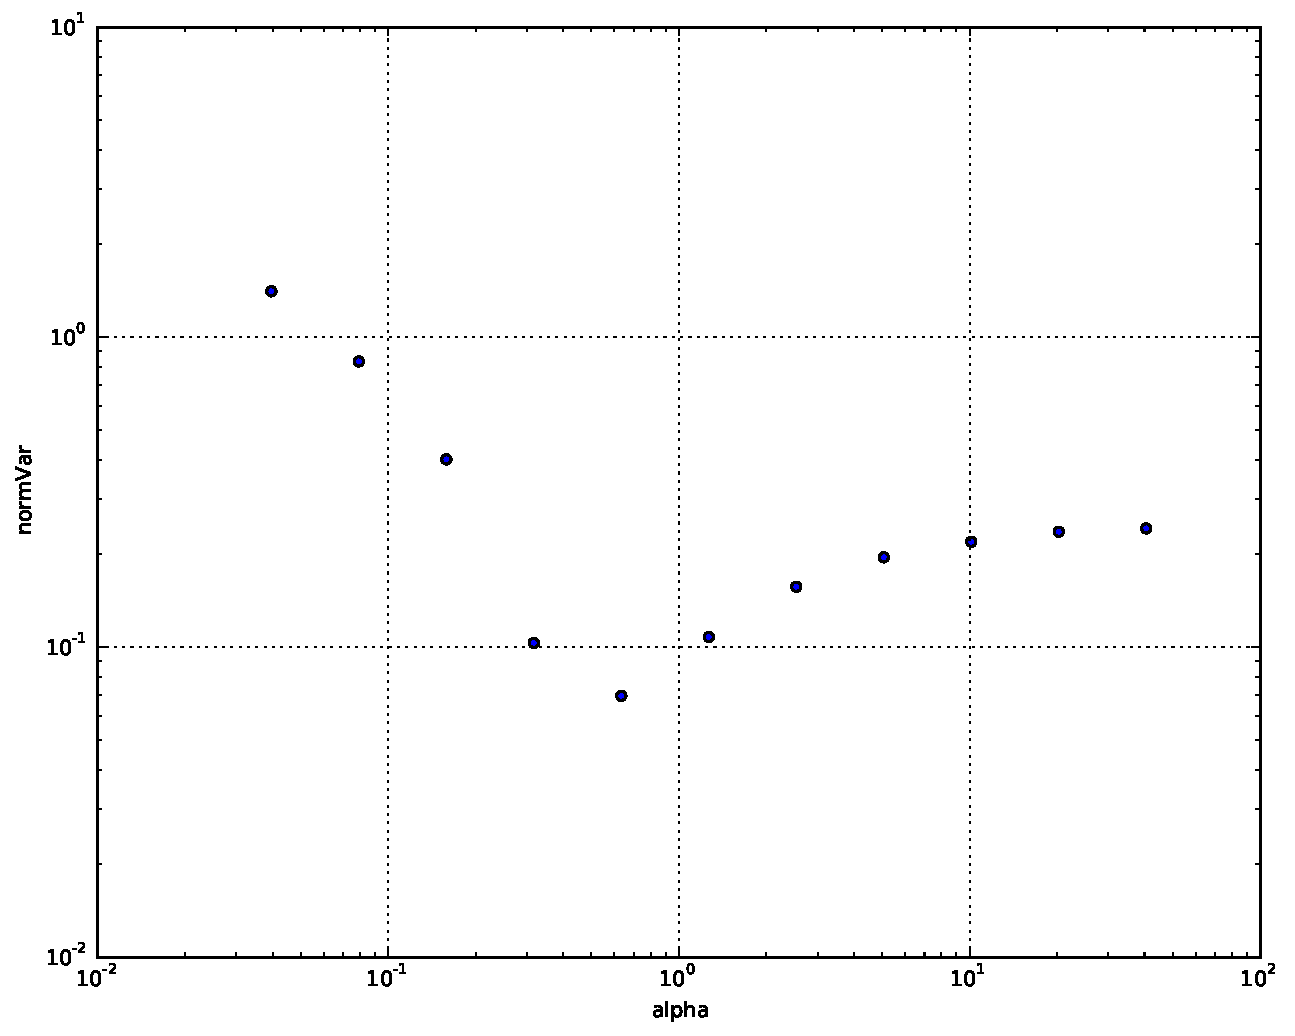
\includegraphics[scale=0.4]{images/minority/alpha_to_norm_var.pdf}
\caption{Plot of normalized variance versus control parameter $\alpha$}
\label{fig:normalized variance}
\end{center}
\end{figure}

Looking at the graph \ref{fig:normalized variance} we can see that for low values of our control parameter $\alpha$ agents perform worse than they would if only random decisions where made.
By incrementing the control parameter, either by raising the memory available or remove certain quantities of agents from the model, the volatility pummels to it's minimum at the critical value of $\alpha$ ($\alpha_c$).
This critical value has been calculated in \cite{marsili2000exact} by Marsili et al. and is equal to $0.3347...$ for $S=2$.
By incrementing further the control parameter the volatility starts incrementing again and converges to the random choice limit.

This behaviour can be observed if we look at the plots of attendance for models with different values of $\alpha$. In figures \ref{fig:attendance_m2}, \ref{fig:attendance_m5} and \ref{fig:attendance_m9} graphs of attendance can be seen for models consisting of $101$ agents but with varying memory size. Different brain sizes plotted here are $2$, $5$ and $9$, which gives us $\alpha$ values of $0.03960$, $0.3168316$ and $5.0693069$ respectively. For $\alpha$ bellow it's critical value we can see that the variance of the attendance is rather high, it becomes minimum for $M=5$ and then again as we increase the brain size it start to have a volatile nature.

\begin{figure}[h]
\begin{center}
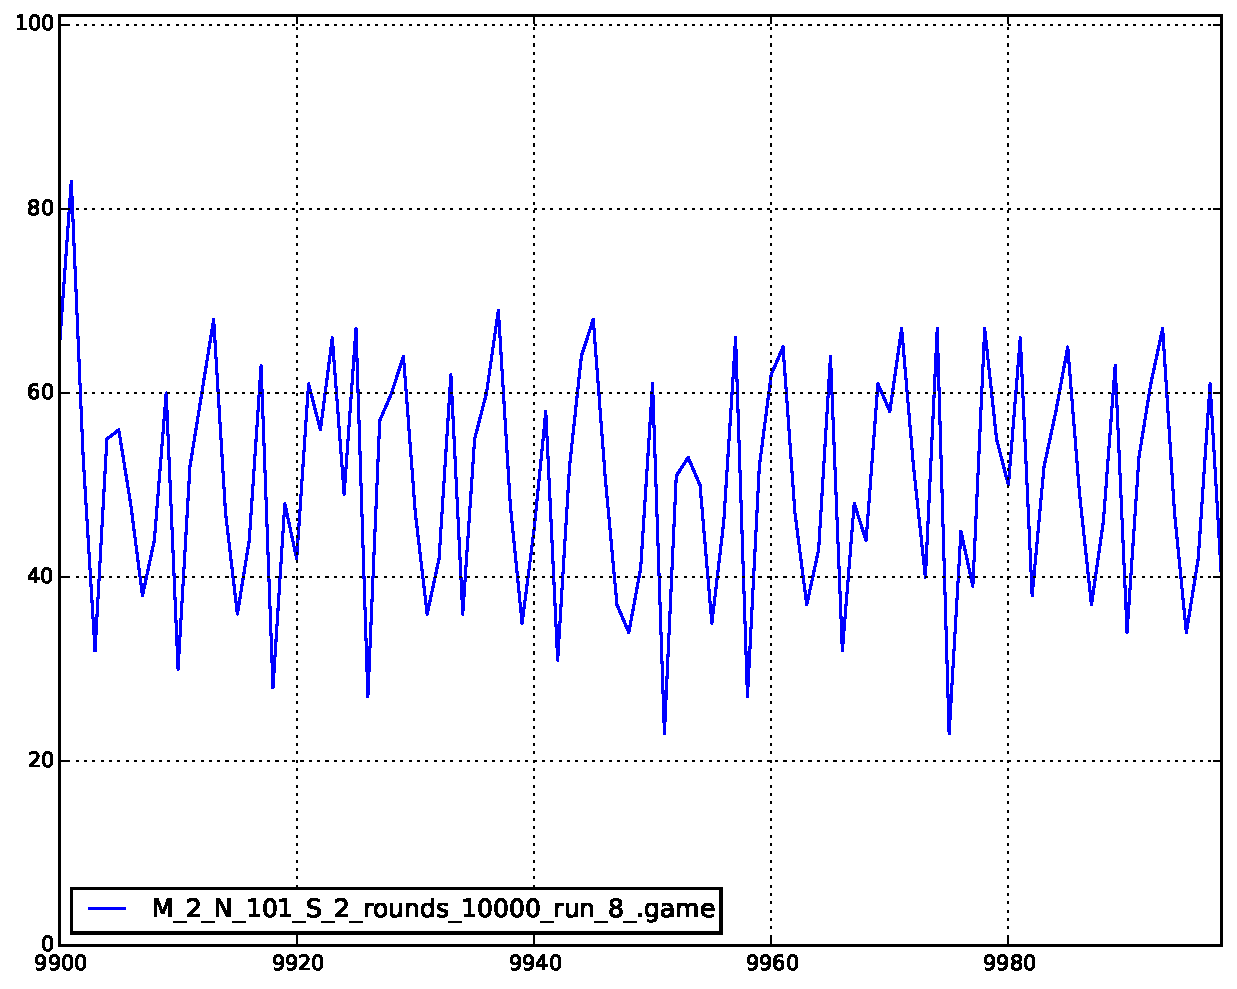
\includegraphics[scale=0.4]{images/minority/attendance_m2_n101.pdf}
\caption{Plot of attendance over time for a model with agents with $M=2$ and $N=101$}
\label{fig:attendance_m2}
\end{center}
\end{figure}

\begin{figure}[h]
\begin{center}
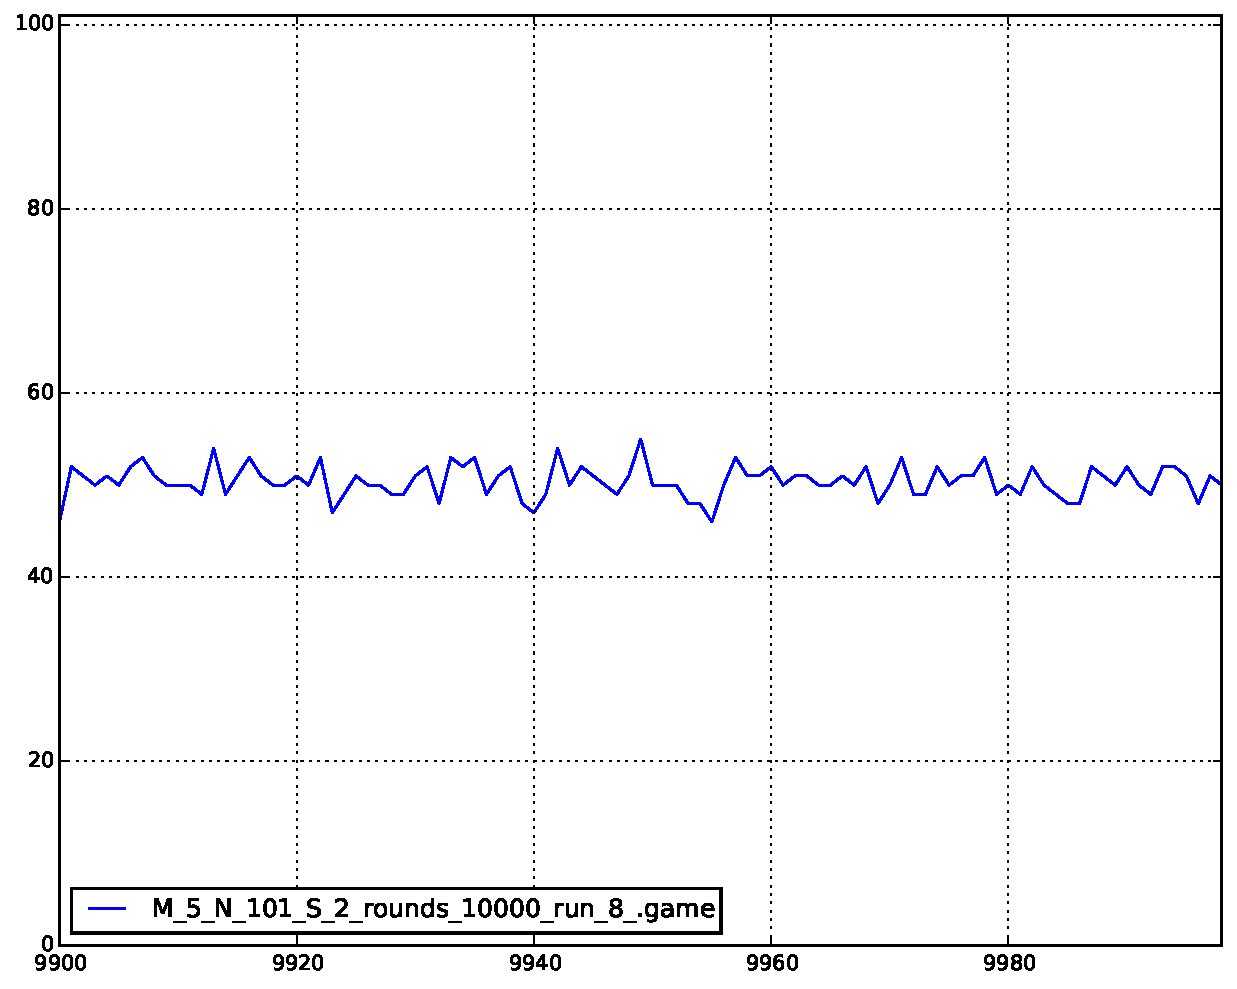
\includegraphics[scale=0.4]{images/minority/attendance_m5_n101.pdf}
\caption{Plot of attendance over time for a model with agents with $M=5$ and $N=101$}
\label{fig:attendance_m5}
\end{center}
\end{figure}

\begin{figure}[h]
\begin{center}
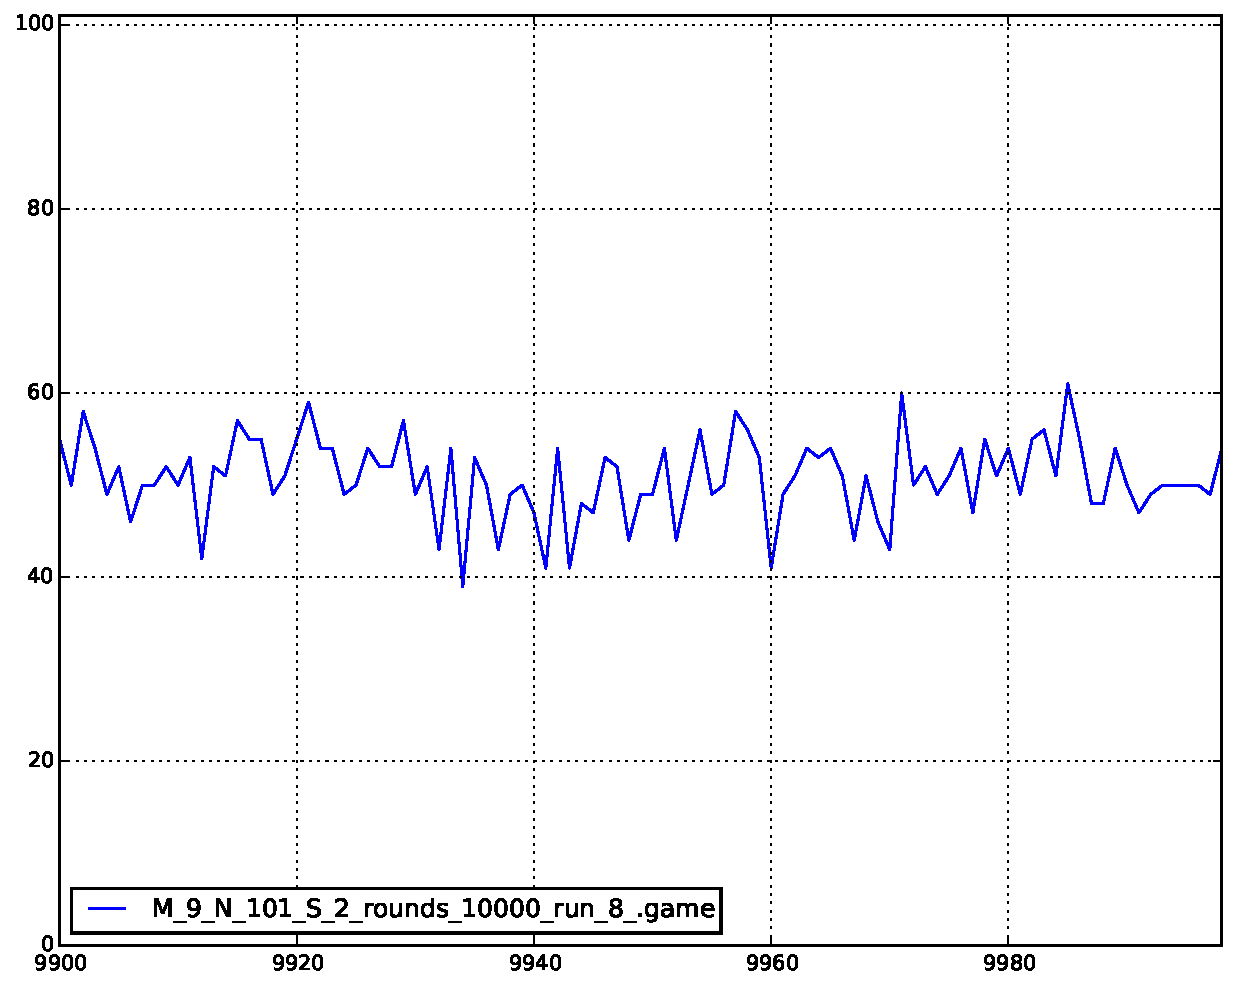
\includegraphics[scale=0.4]{images/minority/attendance_m9_n101.pdf}
\caption{Plot of attendance over time for a model with agents with $M=9$ and $N=101$}
\label{fig:attendance_m9}
\end{center}
\end{figure}

The $\alpha_c$ identifies a separation between two phases of minority games.
To characterize better the two phases let's look at the information available to agents in different phases.
We plot the probability of "1" being the winning choice given a certain history, $P(1|\mu)$ in figures \ref{fig:information_44} and \ref{fig:information_66}.
When the control parameter is below it's critical value $\alpha_c$ the probability of "1" being the winning side is equal to $0.5$ for all values of history $\mu$.
This shows the fact that there is no information to be extracted from the model for agents of that particular brain size for all outcomes seem to be random.
For reasons expressed, this phase is called \textit{unpredictable} phase or also \textit{symmetric} phase for the symmetry present in the histogram of probability given a certain history.
If we look at the graph of probability given a certain history when the control parameter $\alpha$ is above it's critical value, given in figure \ref{fig:information_66}, we can see that there is information available to be exploited in this phase.
This phase hence is called \textit{asymmetric} or \textit{predictable}.
In this phase agents act better than when making random choices, and even though each agent acts in his self best interest we can say that a phenomenon of cooperation emerges as the agents are able to distribute themselves on both sides with rather small variance.
Note that even in the asymmetric phase model retains it's \textit{negative-sum-game} nature and majority of the agents continue to lose, however the number of losing agents is brought to it's minimum.


% probability of 1 given a history
\begin{figure}[h]
\begin{center}
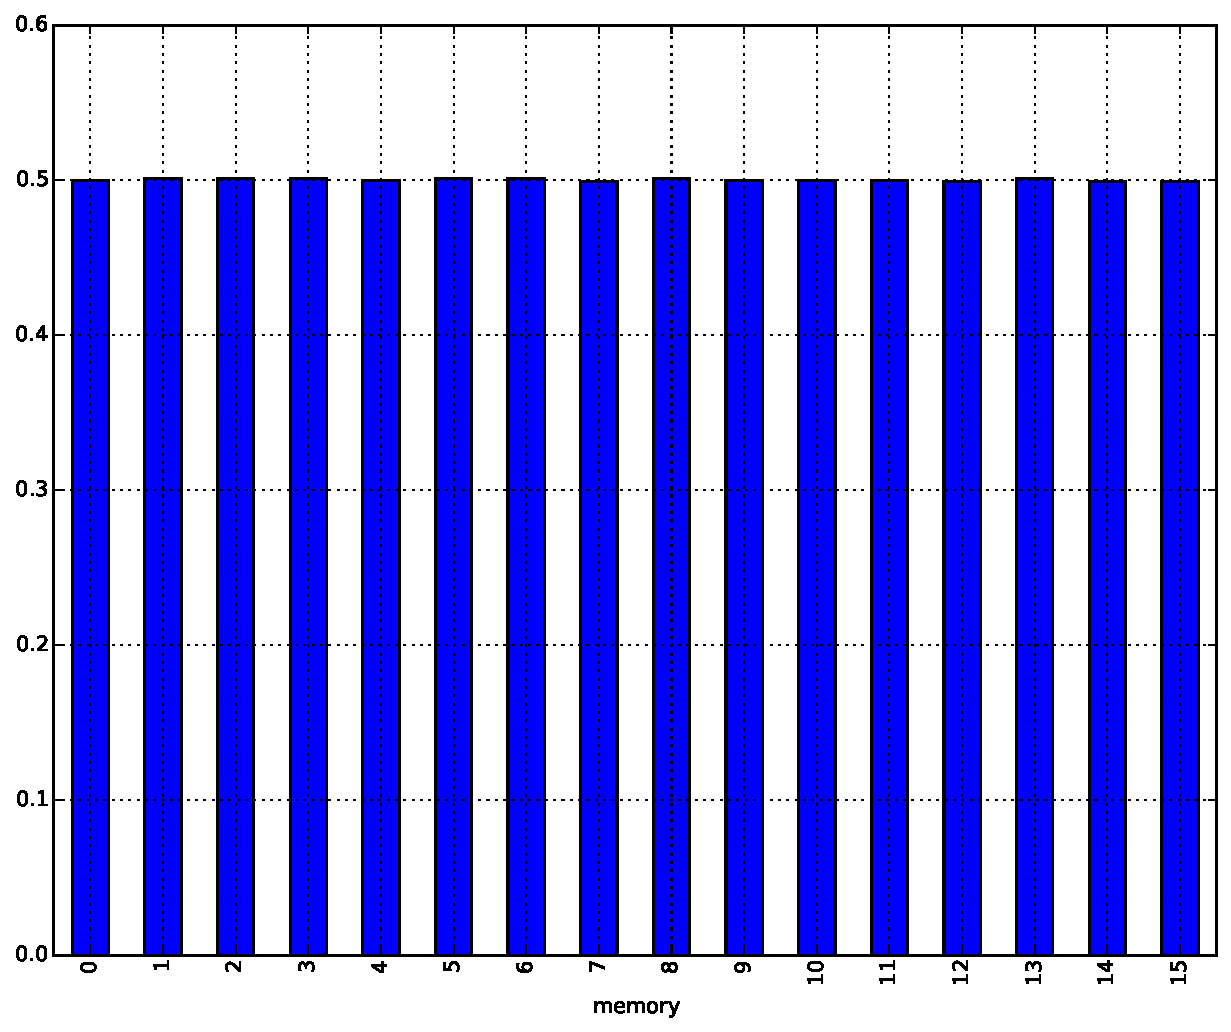
\includegraphics[scale=0.4]{images/minority/information_probability_m4_a4.pdf}
\caption{Plot of $P(1|\mu)$ versus $\mu$ using a sliding window of length $4$ on a model where agents have $M=4$}
\label{fig:information_44}
\end{center}
\end{figure}

\begin{figure}[h]
\begin{center}
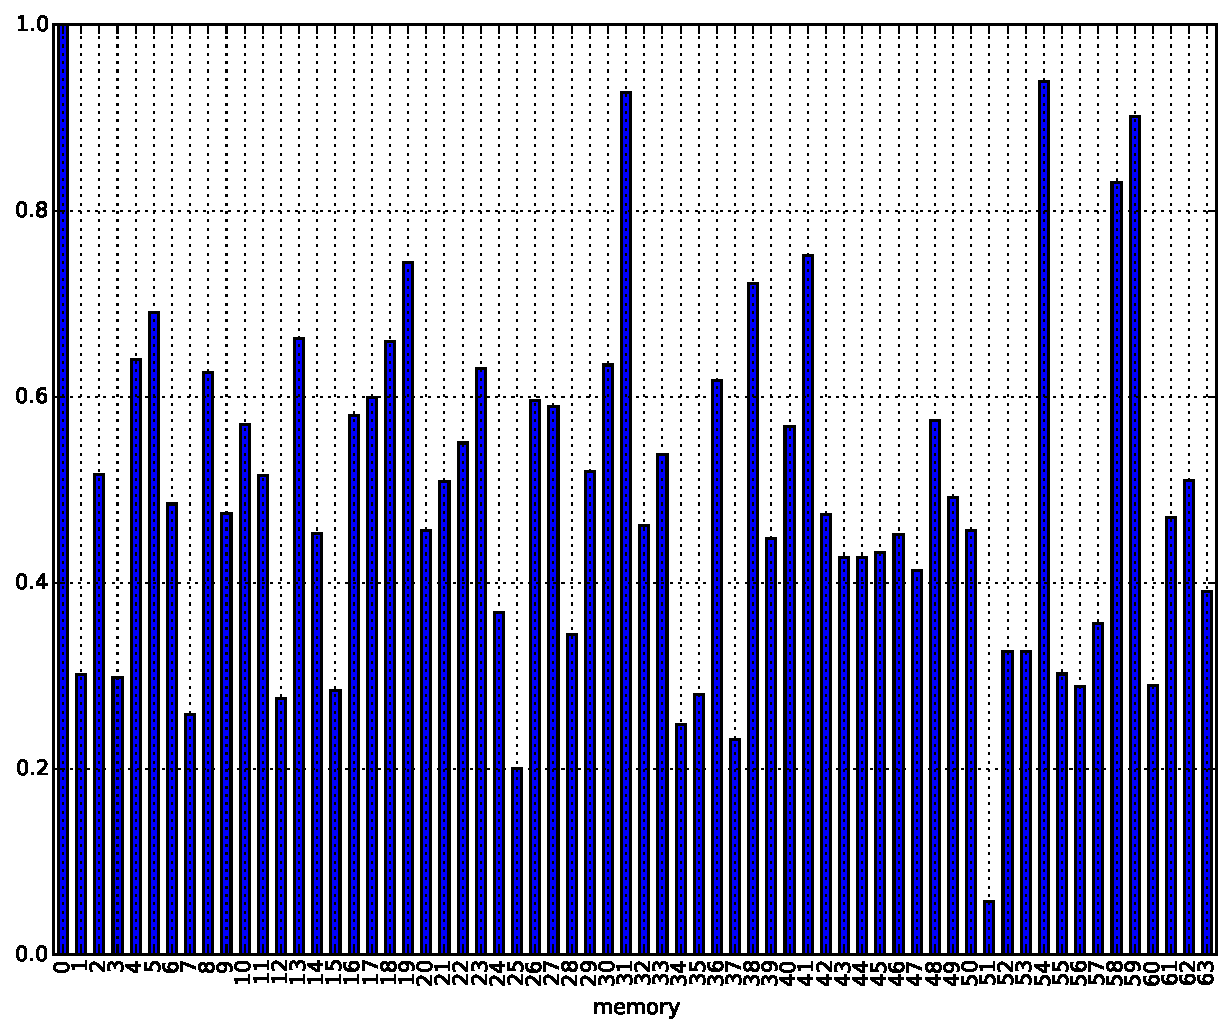
\includegraphics[scale=0.4]{images/minority/information_probability_m6_a6.pdf}
\caption{Plot of $P(1|\mu)$ versus $\mu$ using a sliding window of length $6$ on a model where agents have $M=6$}
\label{fig:information_66}
\end{center}
\end{figure}

It is important to note that the information is present within the model even in the symmetric phase, but the agents don't have the capabilities to exploit that information.
In fact, if we introduce an agent with $M$ greater that those of agents already in the \textit{symmetric} phase we can expect that he will be able to exploit his advantage of greater memory.
The information present in the model for an agent with larger brain size can be seen in figure \ref{fig:information_35} that plots the probability that "1" will be the minority size versus the possible history.

\begin{figure}[h]
\begin{center}
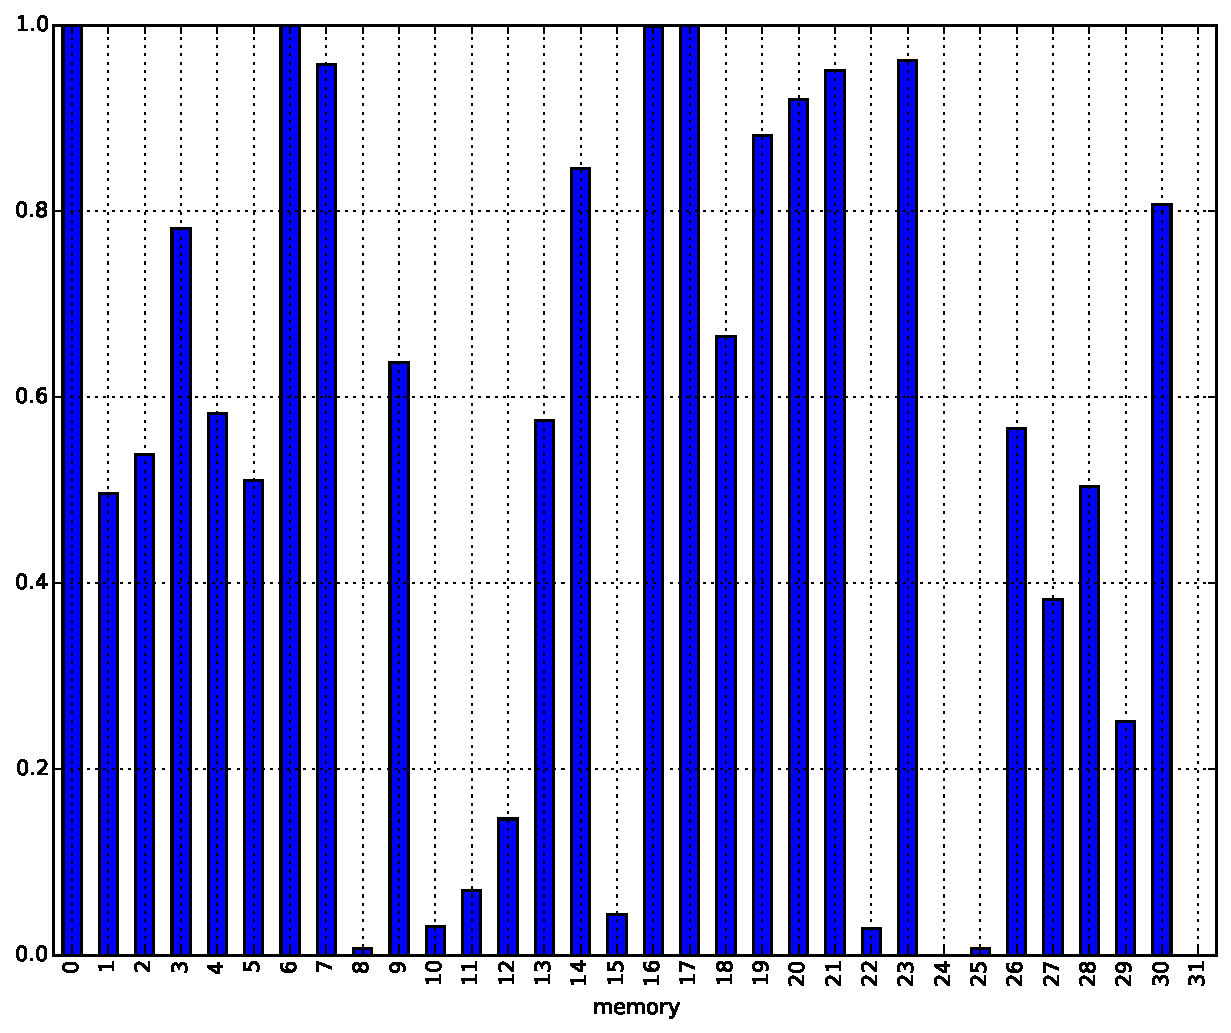
\includegraphics[scale=0.4]{images/minority/information_probability_m3_a5.pdf}
\caption{Plot of $P(1|\mu)$ versus $\mu$ using a sliding window of length $5$ on a model where agents have $M=3$}
\label{fig:information_35}
\end{center}
\end{figure}

\subsection{Crowds and anti-crowds}
\label{subsec:crowds}

The nature of \textit{symmetric} phase brings about the phenomenon of the formation of crowds and anti-crowds.
When we find ourselves in the symmetric phase the $\alpha$ is below it's critical level, meaning that $2^M$ is roughly one order of magnitude smaller than $N$.
The consequence is that the number of available strategies $2^{2^M}$ is low when compared to the number of agents, hence probability of different agents having same strategies is higher than in the \textit{asymmetric} phase.
Another way to explain the phenomenon is to say that when $M$ is low agents are able to efficiently elaborate the information, however since the information is short many agents will come to same predictions, and behave in the same fashion.

The phenomenon of crowds and anti-crowds thus happens in symmetric phase and when it occurs most of the agents behave in the same way, giving rise to high volatility.
If number of agents is large and the number of available strategies is small, it is more opportune to make decisions randomly rather than use deterministic strategies.

\section{Variations for financial markets}
\label{minority:variations}

The basic minority games introduce a very simple model for the financial markets, however there are certain modification to be done before we can start comparing it to a real market.
Let us assume that the action "1" stands for "buy" and action "0" stands for sell.
Attendance can now be seen as a number of agents that participate in the market as buyers, while $N-A(t)$ is the number of sellers.
The quantity $A(t)-\frac{N}{2}$ is the excess demand in the market.
So if that quantity is positive most of the agents involved are buyers and it is profitable at that moment to sell, and viceversa.
This is an economical point of view to the basic mechanism of minority games.
The payoff that is given to agents at each round, introduced in \cite{challet2001stylized}, is defined as
\begin{displaymath}
g_i(t) = =a_i(A(t) - \frac{N}{2})
\end{displaymath}
This captures the fact that the agent on the minority side are awarded proportionally to their investment.

To model the prices Challet et al. have used this price dynamics in their original paper:
\begin{displaymath}
\log p(t+1) = \log p(t) + \frac{A(t)}{\lambda}
\end{displaymath}
where $\lambda$ is related to the market depth.

The most important modification of the basic model when trying to simulate financial markets is the introduction of two types of agents, \textit{producers} and \textit{speculators} that interpret different approaches to the real market.

\subsection{Producers}

Producers, per definition, contribute to the market always following a predetermined behaviour.
They model the agents that produce goods and services, and as such participate in the market at all times.
Since their scope is not to speculate on other agents behaviour but to use market to sell their goods and buy other goods needed, they have a deterministic behaviour, acting always in the same fashion for same values of $\mu(t)$.
Inside the model of the market they create information that is then exploited by speculators.

To model producers starting from our basic model is rather simple, only one strategy is given to the agent and no other changes are made.
Participation is already obligatory in the basic model and having only one strategy makes his deterministic.

\subsection{Speculators}

Speculators on the other hand do not produce goods or services, but use the market to exploit the information injected in the model by the producers to gain profit.
Two main differences between speculators and producers are the facts that speculators have adaptive behaviour and that they can choose not to participate in the market if they find it unprofitable.

In order to model adaptive behaviour $S$ strategies are given to each speculator, drawn randomly from $2^{2^M}$, from which he can choose.
As for the ability to abstain from the market in unfavourable conditions we add yet another strategy, called \textit{0-strategy} that tells the speculator not to interact with the market at chosen time.

At each round the speculator chooses the best strategy by picking the one with the highest virtual score, calculated with:
\begin{displaymath}
U_{i,s}(t+1) = U_{i,s}(t) - [(2a_{i,s}^{\mu(t)}(t+1)-1)(A(t)-\frac{N}{2}) ] + \epsilon\delta_{s_i(t),0}
\end{displaymath}

The first part of the formula is the same as the virtual score calculation for the basic model, ie. a strategy is awarded points if it correctly predicts the minority side.
The second part models the virtual score of the zero strategy that get incremented at every step by $\epsilon$.
This new parameter models the interest rate for the speculators, making them active participants in the market with only the strategies that can guarantee a profit over time that is larger than $\epsilon t$, with t the number of rounds thus far.
Note that all the considerations above with the assumption that $\epsilon$ is positive, in fact if we set $\epsilon$ to be infinitely negative speculators act as agents in the basic model.
